\documentclass[journal]{IEEEtran}
\usepackage{enumerate} 
\usepackage[spanish,activeacute]{babel}
\usepackage{graphicx}
\usepackage[latin1]{inputenc}

\hyphenation{op-tical net-works semi-conduc-tor}


\begin{document}
\title{Contador ascendente y descendente.}
\author{Pedro A. Moreno \\
Departamento de Estudios Multidisciplinarios, Campus Irapuato Salamanca, Universidad de Guanajuato, Yuriria, Guanajuato, M\'exico. \\
Email: pa.morenovazquez@ugto.mx

\thanks{Marzo 14, 2017}}
\markboth{Micrioprocesadores y Microcontroladres,  Febrero~2017}%
{Shell \MakeLowercase{\textit{et al.}}: Bare Demo of IEEEtran.cls for IEEE Journals}



\maketitle

\begin{abstract}

Se obtuvo un contador creciente y decreciente a trav�s de un microcontrolador PIC16F84A, el cual se muestra de forma binaria en  un conjunto de diodos emisores de luz.

\end{abstract}

%\begin{IEEEkeywords}
%IEEE, IEEEtran, journal, \LaTeX, paper, template.
%\end{IEEEkeywords}

\IEEEpeerreviewmaketitle

\section{Introducci\'on }

\IEEEPARstart{E}{l} microncontrolador PIC16F84A puede almacenar registros de hasta 8 bits, lo que se obtienen n�meros del 0 hasta el 255. Un contador creciente incrementa en uno el valor de un registro y el contador decreciente disminuye en 1 el valor del registro.

\section{Metodolog\'ia }

\subsubsection{Materiales}
\begin{itemize}
	\item 1 PIC 16F84A.
    \item 1 mini dip switch de 8 pines.
    \item 8 LED.
    \item 8 resistencias de 300 $\Omega$.
    \item 1 resistencias de 10 $k   {  }\Omega$.
    \item Fuente de alimentaci�n.
\end{itemize}


\subsubsection{Desarrollo}

Para realizar el contador, creciente-decreciente fue necesario el uso de una entrada, switch, la cual definiera si el contador funcionase de forma creciente o de forma decreciente, un registro, REG, en el cual se almacena la operaci�n definida en el switch.
En el proceso primero se mostraba lo contenido en el registro posteriormente se llamaba una rutina de tiempo, de 90909 microsegundos, para que el usuario distinguiera el incremento o decremento, se sigui� por revisar el estado de la entrada y decidir as� que operaci�n ejecutar.

\begin{figure}
  \centering
    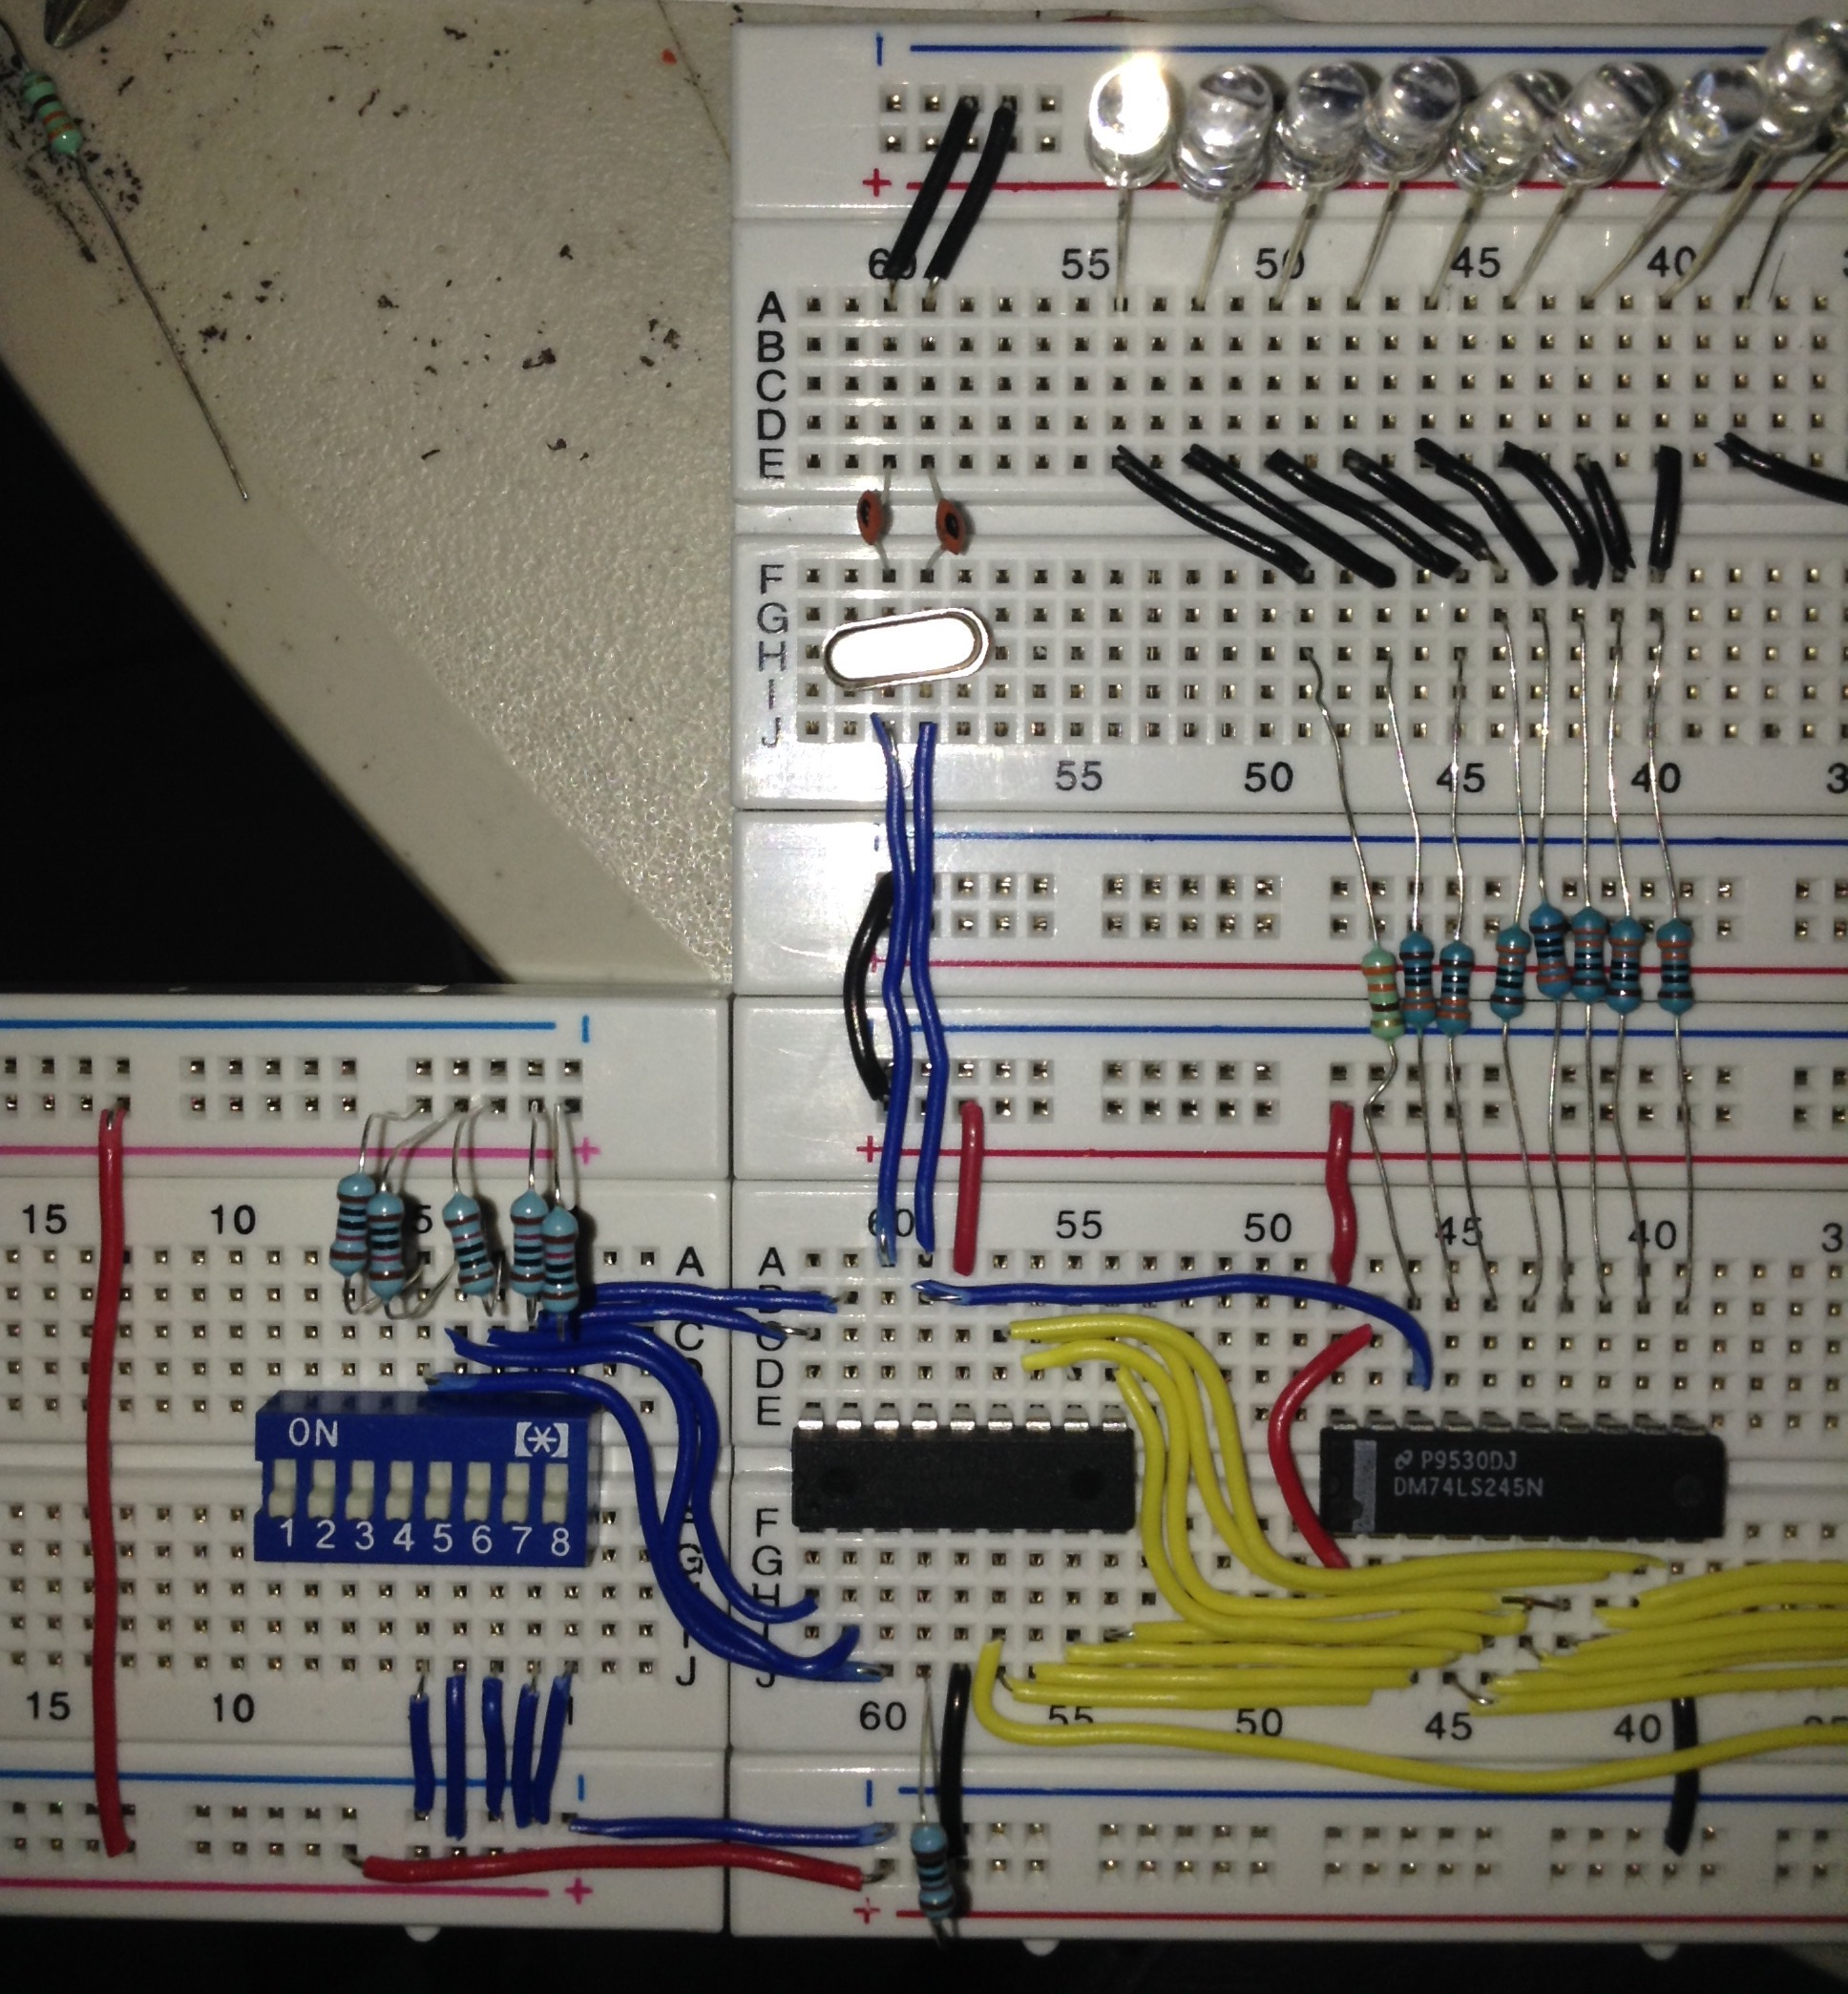
\includegraphics[width=0.45\textwidth]{FullSizeRender2.jpg}
  \caption{Circuito.}
  \label{calentrada}
\end{figure}




 
\section{Resultados }

En el conjunto de LEDs, se apreciaba el incremento y decremento de un valor en forma binaria, esto fue posible gracias al uso de la rutina de tiempo y las funciones para incrementar o decrementar contenidas en el PIC.

\section{Conclusi\'on }
Con los microcontroladores se es capaz de obtener contadores los cuales pueden tener diversas aplicaciones, como la mas que com�n que es ser el pilar de una rutina de tiempo.



\end{document}